\newcommand{\bmop}{\mathcal{G}}

\chapter{Hybrid finite/boundary element method}
\chaptermark{Hybrid FEM/BEM}
\label{sec:hybr-finit-elem}

The boundary element method (BEM) is a spatial discretisation method similar to the FEM except that the problem on a domain is converted to an equivalent formulation in terms of integrals over the boundary of the domain before the discretisation is applied.
The main downside of such a formulation is that it results in a dense matrix after the discretisation is applied.

The hybrid finite/boundary element method (FEM/BEM) is a spatial discretisation method which applies FEM and BEM to different parts of the same problem.
In particular this method can be applied in the context of magnetostatic calculations to enforce the boundary condition at infinity in \cref{eq:cont-phi-bound} without meshing an infinite region of space or arbitrarily truncating it.
This is done by applying the BEM to a part of the problem on the infinite external domain in order to convert it into a problem on the boundary of the magnetic domain.
The use of FEM for the remaining parts of the problem means that most of the obtained linear systems remain sparse.

In \thisref{sec:hybr-finit-elem} we first give an overview of the FEM/BEM approach and then show how splitting the magnetostatic problem into two parts and applying some results from potential theory can lead to a formulation which involves only finite domains.
We then demonstrate how this formulation can be discretised, and discuss the evaluation of the required integrals.
Methods of coupling the FEM/BEM magnetostatic calculations to the FEM-discretised LLG problem (as described in \cref{sec:galerk-meth-llg}) are discussed in \cref{sec:solution-strategies}, along with strategies for the solution of the resulting linear/non-linear systems.


\section{The continuous FEM/BEM formulation}
\label{sec:bem-derivation}


 % I'm worried about whether all this is ok with weak form: we use strong form for derivation of boundary formulation then ``just assume'' that it will all be ok when we weak form it...
% But since, in the final equations, there are no derivatives of the solution we should be ok right?
% It must be ok somehow because people use Galerkin BEM! Just need to read the book to see why

We want to use the boundary element method in the calculation of the magnetostatic scalar potential, $\phim$, (defined in \cref{eq:Hms,eq:cont-phi-bound}) to avoid performing calculations that involve the infinite external domain.
However, applying the boundary element method alone would require the solution of dense matrix equations for the entire problem.
We can circumvent this issue by applying a hybrid method using both FEM and BEM.
We use the linearity of the Poisson operator to split the potential into two parts $\phim = \phione + \phitwo$ in such a way that $\phione$ can be calculated in the magnetic domain, $\magd$, using only the finite element method.
This results in conditions on $\phitwo$ that must be satisfied to give the correct total potential, including the problematic condition at infinity.

It turns out that $\phim$ can be split in such a way that the $\phitwo$ is equivalent to the potential resulting from a specific arrangement of fictional magnetic charges, which is known to solve the required differential equation including the boundary condition at infinity.
The details of this ``charge distribution'', which gives rise to a double-layer potential, depend on the boundary values of $\phione$.
The use of such a charge distribution is equivalent to applying the BEM to $\phitwo$.

So given $\phione$ and using the known solution for this charge distribution we can calculate $\phitwo$ anywhere.
However the calculation of $\phitwo$ at a point using this method involves an expensive dense matrix operation, so we only use it to calculate Dirichlet boundary conditions for $\phitwo$ on the boundary of the magnetic domain, $\boundd$.
These boundary conditions allow us to apply the finite element method to find $\phitwo$ inside the magnetic domain $\magd$ using standard sparse matrix techniques.

The magnetostatic field $ \hms = \grad \phim$ constructed by the procedure outlined above is \emph{the} magnetostatic field by the uniqueness (up to a constant) of solution for Poisson's equation with Dirichlet or Neumann boundary conditions.\footnote{To see the uniqueness take the difference of two solutions of Poisson's equation: $\phi = \psi_1 - \psi_2$.
Then using identity \cref{eq:20}, the linearity of Poisson's equation and the divergence theorem we obtain $\intb{\phi \grad \phi \cdot \nv} = \intd{(\grad \phi)^2 }$.
Applying Dirichlet, Neumann or mixed boundary conditions shows that the boundary integral is zero and hence $\grad \phi = 0$.}

In \cref{sec:problem-description} we describe in more detail the splitting of the potential that allows this process.
Then in \cref{sec:double-layer-potent} we describe the properties of the fictional charge distribution.
Finally in \cref{sec:appl-magn-calc} we combine these parts to give a formulation of the magnetostatic problem involving only finite sized domains.

\subsection{The potential splitting}
\label{sec:problem-description}
\newcommand{\examplepot}{f}

\begin{figure}
  \center
  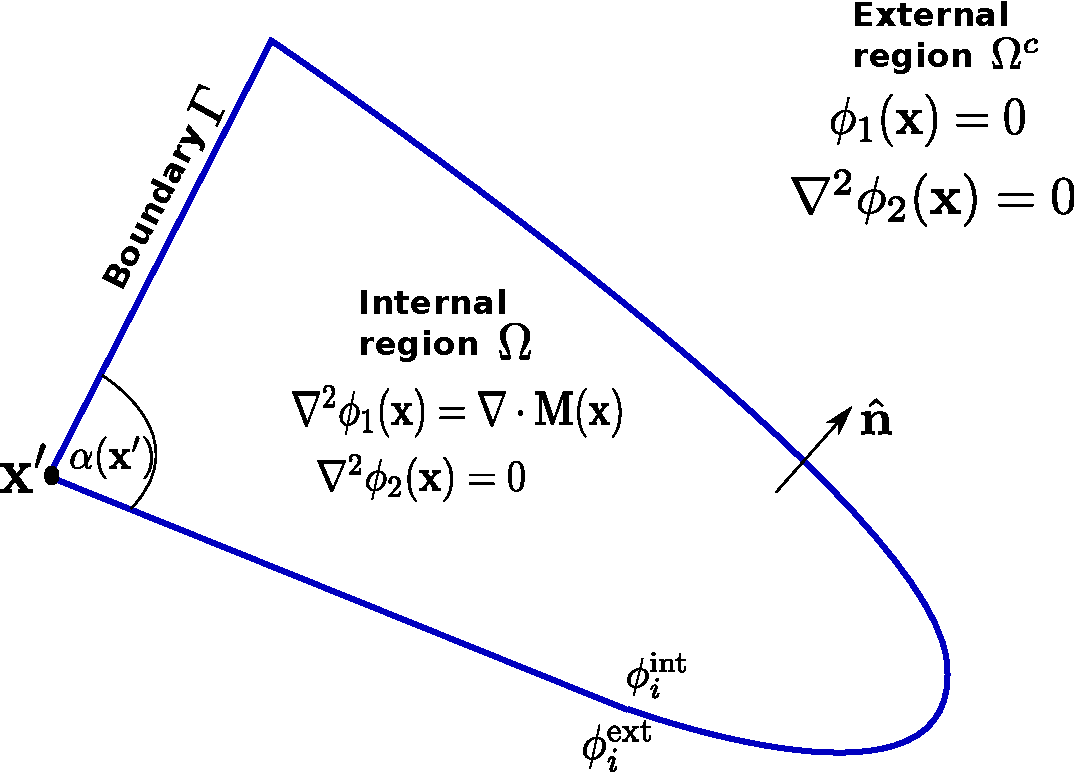
\includegraphics[width=0.75\textwidth]{./images/BEM-geometry}
  % \begin{tikzpicture}

  %   %   Main nodes and some labels
  %   \node[label=below:$\xv'$] (a) at (-2,-2) {};
  %   \node (b) at (-2,2) {};
  %   \node[label=right:\Large{$\boundd$}] (c) at (5,0) {};

  %   %   Draw main shape of magnetic domain
  %   \draw [line width=0.5mm,draw=solidblue,fill=paleblue] (a.north) to [bend right=71] (c) to (b.south);
  %   \draw [line width=0.5mm,draw=solidblue] (a) to (b);
  %   \draw (a.north) circle(1mm) [fill=black] {};

  %   %   More labels
  %   \node (center) at (1,0) {\Large{Magnetic domain $\magd$}};
  %   \node(external) at (8,3) {\Large{External domain $\extd$}};
  % \end{tikzpicture}

  \caption{A 2D representation of the geometry showing the labels used in \thisref{sec:hybr-finit-elem}.
    The point $\xv'$ is a singular point of the boundary $\boundd$, the angle $\alpha(\xv')$ is as shown.}
  \label{fig:BEM-geometry}
\end{figure}

First we need to introduce some notation: we write $\examplepot^\inte(\xv) = \lim_{\xv \rightarrow \boundd} \examplepot(\xv)$ from inside the magnetic domain, $\examplepot^\exte(\xv) = \lim_{\xv \rightarrow \boundd} \examplepot(\xv)$ from outside the magnetic domain.
That is, $\examplepot^\inte$ denotes the value of $\examplepot$ ``close'' to the boundary $\boundd$ and ``just inside'' the magnetic domain and $\examplepot^\exte$ for the value of $\examplepot$ ``just outside'' the magnetic domain (see \cref{fig:BEM-geometry}).

From \cref{sec:magnetostatic-field} we have certain \emph{physical} conditions on the magnetostatic potential $\phim$.
Both inside and outside the magnetic domain, $\magd$, we have
\begin{equation}
  \lap \phim(\xv) = \div \mv(\xv),
  \label{eq:2}
\end{equation}
where we define $\mv = \zerov$ outside of magnetic materials.
We also have the boundary conditions
\begin{equation}
  \pd{\phim^\inte(\xv)}{\nv} - \pd{\phim^\exte(\xv)}{\nv} = \mv \cdot \nv \qquad \xv \in \boundd,
  \label{eqn:dphibound}
\end{equation}
and
\begin{equation}
  \phim^\inte(\xv) - \phim^\exte(\xv)  = 0 \qquad \xv \in \boundd,
  \label{eqn:phibound}
\end{equation}
on the boundary of the magnetic material, $\boundd$.
Finally we have the condition that
\begin{equation}
  \phim(\xv) \rightarrow 0 \qquad \text{ as } \abs{\xv} \rightarrow \infty.
  \label{eq:48}
\end{equation}
Note that \cref{eqn:dphibound,eqn:phibound} imply continuity but not smoothness of the magnetic potential $\phim$ across $\boundd$. This effect can be thought of as the effect of (fictional) surface monopole charges.

The key observation for this part of the derivation is that \cref{eq:2,eq:48,eqn:dphibound,eqn:phibound} are linear, \ie if $\phim = \phione + \phitwo$ then $\lap \phim = \lap \phione + \lap \phitwo$ and similarly for the boundary conditions.
Based on this observation we define a new potential $\phione$ which satisfies
\begin{equation}
  \phim(\xv) = \phione(\xv) + \phitwo(\xv),
  \label{eq:21}
\end{equation}
everywhere in $\real^d$ and
\begin{equation}
  \lap \phione(\xv) = \div \mv(\xv) \qquad \xv \in \magd,
  \label{eq:1}
\end{equation}
\begin{equation}
  \pd{\phione^\inte(\xv)}{\nv} = \mv \cdot \nv \qquad \xv \in \boundd,
  \label{eqn:dphionebound}
\end{equation}
\begin{equation}
  \phione(\xv) = 0 \qquad \xv \in \extd,
  \label{eqn:phioneoutside}
\end{equation}
where $\extd = \real^d \backslash \magd$ is the infinite region of free space outside the magnetic domain.
Note that \cref{eq:1,eqn:dphionebound} give a self contained Poisson Neumann problem for $\phione \in \magd \cup \boundd$, and that \cref {eqn:phioneoutside} implies
\begin{equation}
  \pd{\phione^\exte(\xv)}{\nv} = 0 \qquad \xv \in \boundd.
  \label{eq:32}
\end{equation}


\Cref{eq:2,eq:48,eqn:dphibound,eqn:phibound} for $\phim$ combined with \cref{eq:21,eq:1,eqn:dphionebound,eqn:phioneoutside} for $\phione$ give a number of conditions that $\phitwo$ must satisfy.
From \cref{eq:2,eq:21,eq:1} and the fact that the problem is linear we have a differential equation for $\phitwo$:
\begin{equation}
  \label{eq:8}
  \lap \phitwo(\xv) = 0,
\end{equation}
everywhere in $\real^d$.
Substituting \cref{eq:21} into \cref{eqn:dphibound} and using \cref{eqn:dphionebound,eq:32} gives
\begin{equation}
    \pd{\phitwo^\inte(\xv)}{\nv} - \pd{\phitwo^\exte(\xv)}{\nv} =
    \pd{\phione^\exte(\xv)}{\nv} - \pd{\phione^\inte(\xv)}{\nv}
    + \mv \cdot \nv \qquad \xv \in \boundd,
\end{equation}
thus the first boundary condition on $\phitwo$ is
\begin{equation}
  \pd{\phitwo^\inte(\xv)}{\nv} = \pd{\phitwo^\exte(\xv)}{\nv}  \qquad \xv \in \boundd.
  \label{eq:5}
\end{equation}
Finally from \cref{eqn:phibound,eq:21,eqn:phioneoutside} we have a second boundary condition on $\phitwo$:
\begin{equation}
  \begin{aligned}
    (\phione^\inte + \phitwo^\inte) - (\phione^\exte + \phitwo^\exte) &= 0, \\
    \phitwo^\inte - \phitwo^\exte &= - \phione^\inte &\qquad \xv \in \boundd.
    \label{eq:4}
  \end{aligned}
\end{equation}
As mentioned previously, the solution of the Laplace equation \cref{eq:8} subject to the boundary conditions \cref{eq:5,eq:4} is satisfied by a certain arrangement of virtual magnetic charges.
This arrangement of charges is discussed in the next section.

\subsection{Double Layer Potentials}
\label{sec:double-layer-potent}

A double layer potential can be thought of as the potential due to a layer of dipoles (\ie two charges separated by an infinitesimal distance) of magnitude $\mu(\xv)$ in direction $\nv$ over the surface $\boundd$ \cite{Sternberg1946}.\footnote{Note that our potentials are a factor of $\frac{-1}{4 \pi}$ different from those in reference \cite{Sternberg1946} and that our $\phim^\inte$ and $\phim^\exte$ definitions correspond to their $\phim^-$ and $\phim^+$.}
In \thisref{sec:double-layer-potent} we give some (mathematical) properties of a double layer potential.
%, in \cref{} we will demonstrate that we can use a double layer potential to calculate $\phitwo^\inte$ in terms of $\phione^\inte$.

The double layer potential at a point $\xv \in \real^d$ (including $\xv \in \boundd$) is defined as
\begin{equation}
  \label{eq:3}
  \phim(\xv) = \int_{\boundd} \mu(\yv) \pd{\Green}{\nv(\yv)} \d \yv,
\end{equation}
where $G$ is the Green's function for a Laplacian operator and $\nv(\yv)$ is the outward unit normal at $\yv \in \boundd$.
For $d=2$
\begin{equation}
  \Green = \dfrac{-1}{2\pi}\ln(\abs{\xv - \yv}),
  \label{eqn:greenslaplacian2d}
\end{equation}
and for $d=3$
\begin{equation}
  \Green = \dfrac{-1}{4 \pi} \dfrac{1}{\abs{\xv - \yv}}.
  \label{eqn:greenslaplacian3d}
\end{equation}


We have the following results from potential theory:
\begin{enumerate}
\item The double layer potential satisfies Laplace's equation $\lap \phi = 0$ (in other words the double layer potential is harmonic) \cite{Sternberg1946}.

\item The double layer potential undergoes a jump of $\mu(\xv)$ moving in the direction $\nv$ across a smooth surface $\boundd$ \cite[136-140]{Sternberg1946}, \ie
  \begin{equation}
    \label{eq:15}
    \phim^\inte(\xv) - \phim^\exte(\xv) = \mu(\xv).
  \end{equation}

\item Defining the fractional angle at a point as
  \begin{equation}
    \gamma(\xv) = \frac{\alpha(\xv)}{\alpha_{\text{max}}},
  \end{equation}
  where, in two dimensions, $\alpha(\xv)$ is the angle subtended by the domain at $\xv$ and $\alpha_{\text{max}} = 2\pi$.
  Similarly in three dimensions $\alpha(\xv)$ is the solid angle and $\alpha_{\text{max}} = 4\pi$.

  Then for $\xv \in \boundd$ the following relationship holds \cite[137-139, 155]{Sternberg1946}
  \begin{equation}
    \phim^\inte(\xv) = (1 - \gamma(\xv)) \mu(\xv) + \phim(\xv).
    \label{eq:22}
  \end{equation}
  Note that the angle $\alpha$ at a ``smooth'' point\footnote{The surface must be a Lyapunov surface at the point.
This means that ??ds
\cite{??ds}} on the surface is $\pi$ in 2D (or $2\pi$ in 3D).
  So in these cases $\gamma(\xv) = \frac{\alpha(\xv)}{\alpha_{\text{max}}} = \frac{1}{2}$.

\item If $\mu$ is continuous and has continuous first and second derivatives along the boundary (\ie $\mu(\xv) \in C^2(\boundd)$) then the limits $\pd{\phim^\inte(\xv)}{\nv}$ and $\pd{\phim^\exte(\xv)}{\nv}$ exist and are equal \cite[145-153]{Sternberg1946}.

\end{enumerate}

Note that some derivations of the results above rely on the surface being a Lyapunov surface which imposes a number of smoothness conditions on the surface, in particular excluding surfaces with corners.
The proofs given in \cite{Sternberg1946} allow a finite number of sharp corners, \ie a polygonal domain.

\subsection{Application to Magnetostatic Calculations}
\label{sec:appl-magn-calc}

From \cref{sec:double-layer-potent} we can see that conditions \cref{eq:8,eq:5,eq:4} on $\phitwo$ are satisfied by a double layer potential with magnitude\footnote{It is also possible to directly derive the double layer potential formula from \cref{eq:8,eq:5,eq:4}, as described in \cite[Appendix 2]{Knittel2011}.}
\begin{equation}
  \label{eq:24}
  \mu(\xv) = - \phione^\inte(\xv).
\end{equation}

By the uniqueness of solution for Poisson's equation this gives us, up to an additive constant, the only solution for $\phitwo(\xv)$ in the external domain.
This is good enough for a potential since it is only used in $\hms(\xv) = - \grad \phim(\xv)$ and addition of a constant has no effect.

Substituting \cref{eq:24} into \cref{eq:3,eq:22} we have:
\begin{equation}
  \label{eq:6}
  \phitwo^\inte(\xv) =
  - \int_{\boundd} \phione^\inte(\yv) \pd{\Green}{\nv(\yv)} \d \yv
  + \big(\gamma(\xv) - 1 \big) \phione^\inte(\xv).
\end{equation}
After substituting our definition for the three dimensional Green's function \cref{eqn:greenslaplacian3d} into \cref{eq:6} we obtain the same equation as given by Koehler et. al. \cite{Koehler1997}.

Also note that $\phim = \phione + \phitwo$ everywhere, so
\begin{equation}
  \begin{aligned}
    \label{eq:18}
    \phim^\inte(\xv)
    &= - \int_{\boundd} \phione^\inte(\yv) \pd{\Green}{\nv(\yv)} \d \yv
    + \gamma(\xv) \phione^\inte(\xv).
  \end{aligned}
\end{equation}
Either \cref{eq:6} or \cref{eq:18} can be used to give boundary conditions for $\phitwo \in \magd$ or $\phim \in \magd$ respectively.
We will proceed using \cref{eq:18} since it eliminates $\phitwo$ from later calculations and is slightly simpler.
We also omit the distinction between interior and exterior since all exterior values have now been eliminated.

The final continuous problem is
\begin{equation}
  \begin{aligned}
    \lap \phim(\xv) &= \div \mv(\xv),  \\
    \lap \phione(\xv) &= \div \mv(\xv),
  \end{aligned}
  \label{eq:phi-bem-continuous}
\end{equation}
in the magnetic domain $\magd$, with boundary conditions
\begin{equation}
  \begin{aligned}
    \phim(\xv) &= \bmop \big[ \phione(\xv) \big]      & \xv \in \boundd, \\
    \pd{\phione(\xv)}{\nv} &= \mv \cdot \nv  & \xv \in \boundd,
    \label{eq:phi-bem-continuous-bc}
  \end{aligned}
\end{equation}
where the operator $\bmop$ is defined as
\begin{equation}
  \bmop \bigs{\phione(\xv)} = - \int_{\boundd} \phione(\yv) \pd{\Green}{\nv(\yv)} \d \yv
  + \gamma(\xv) \phione(\xv).
\end{equation}
Note that $\phione$ has purely Neumann boundary conditions, hence it is only defined up to a constant.
However, as mentioned before, the addition of a constant is not important so we can fix $\phione$ to zero at some point to resolve this issue.

So if $\mv$ is some fixed function, we can apply the FEM to calculate $\phione$, then use $\bmop$ (assuming we have some discrete version of it) to calculate Dirichlet boundary conditions on $\phim$ and, finally, use the FEM again to calculate $\phim$.
However, in the context of an implicit time integration scheme applied to the LLG equation the value of $\mv$ is not fixed, and entire problem should be solved simultaneously to find a consistent set of $\mv$, $\phione$ and $\phim$.
Efficient methods for the solution of such a simultaneous system, or methods which avoid it, are the topic of \cref{sec:solution-strategies}.
For now we continue by showing how the problem can be discretised.

\section{Discretisation}
\label{sec:discretisation}

% Just in case we do need to distinguish between phim and phione basis functions:
\newsubcommand{\tbfone}{\tbf}{}
\newsubcommand{\tbfm}{\tbf}{}

The bulk equations~\cref{eq:phi-bem-continuous} and the Neumann boundary condition on $\phione$ in \cref{eq:phi-bem-continuous-bc} are identical to those discussed in \cref{sec:llg-initial-equations} and will be solved using the finite element method.
As such the weak residual form, discretisation and Jacobians are identical and all that remains to be discretised is the operator $\bmop$.
We let
\begin{equation}
  \phim = \sum_\ibasis \phim_{\ibasis} \tbfm_{\ibasis}(\xv),
  \qquad
  \phione = \sum_\ibasisb \phione_{\ibasisb} \tbfone_{\ibasisb}(\xv),
  \label{eq:25}
\end{equation}
where $\tbf_i$ are the same polynomial basis functions as used in the finite element method of \cref{sec:galerk-meth-llg}.

Substituting \cref{eq:25} into \cref{eq:18} we have
\begin{equation}
  \sum_\ibasis \phim_{\ibasis} \tbfm_{\ibasis}(\xv) =
  - \int_{\boundd} \sum_\ibasisb \phione_{\ibasisb} \tbfone_{\ibasisb}(\yv)
  \pd{\Green}{\nv(\yv)} \d \yv
   + \gamma(\xv) \sum_\ibasisb \phione_{\ibasisb} \tbfone_{\ibasisb}(\xv).
\end{equation}

Since the integrands are continuous functions on $\boundd$, we can exchange the order of the sum and the integration, leaving
\begin{equation}
  \sum_\ibasis \phim_{\ibasis} \tbfm_{\ibasis}(\xv) =
  - \sum_\ibasisb  \phione_{\ibasisb}  \bigs{\int_{\boundd} \tbfone_{\ibasisb}(\yv)
    \pd{\Green}{\nv(\yv)} \d \yv }
  + \gamma(\xv) \sum_\ibasisb \phione_{\ibasisb} \tbfone_{\ibasisb}(\xv).
  \label{eq:27}
\end{equation}

At this point we could apply the Galerkin method (as described in \cref{sec:intr-finite-ele-diff}): by multiplying \cref{eq:27} by a test function and integrating.
This would result in a system of linear equations $\Mm \phimdis = \bm' \phionedis$ (where $\bm'$ is the Galerkin discrete form of $\bmop$) which could be solved for $\phimdis$.
However this would require calculating a double integral for each entry in $\bm'$.
Instead we apply a standard collocation method.
Collocation methods enforce pointwise relationships in contrast to the Galerkin method which enforces relationships in a weighted integral form.
The collocation method is the conventional choice of discretisation approach for the BEM operator in micromagnetics.

To get the value of $\phim$ at node $\ibasisc$ using the collocation method we choose $\xv = \xv_\ibasisc$ in \cref{eq:27}.
Then using the property $\tbf_\ibasis(\xv_\ibasisc) = \delta_{\ibasis \ibasisc}$ and replacing $\ibasisc$ by $\ibasis$ we have
\begin{equation}
  \phim_{\ibasis} =
  - \sum_\ibasisb \phione_{\ibasisb}  \bigs{\int_{\boundd_\ibasisb} \tbfone_{\ibasisb}(\yv)
  \pd{\Green[\ibasis]}{\nv(\yv)} \d \yv}
   + \gamma(\xv_\ibasis) \phione_{\ibasis},
  \label{eq:colocation}
\end{equation}
where ${\boundd_\ibasisb}$ is the region of $\boundd$ where $\tbfone_{\ibasisb} \neq 0$, \ie the elements which contain node $\ibasisb$.
Notice that the expression inside the square brackets is independent of all potentials: it depends only on the geometry and so can be pre-calculated and stored.


The equation \cref{eq:colocation} gives the value of $\phim$ at a boundary node in terms of a sum of geometric factors multiplied by the values of $\phione$ at each boundary node.
In other words, this is a multiplication by a dense matrix $\bm$ giving $\phim$ at all the boundary nodes in terms of $\phione$ at all boundary nodes:
\begin{equation}
  \label{eq:10}
  \phimdis = \bm \phionedis,
\end{equation}
where
\begin{equation}
  \label{eq:17}
  \bm_{\ibasis\ibasisb} = - \int_{\boundd_\ibasisb} \tbfone_{\ibasisb}(\yv) \pd{\Green[\ibasis]}{\nv(\yv)} \d \yv
   + \gamma(\xv_\ibasis)\delta_{\ibasis\ibasisb}.
\end{equation}

% ??ds this might be wrong in powers in denom.. check  -- Andrew
We now convert the normal derivative of the Green's function into a more tangible form.
In 3D
\begin{equation}
  \label{eq:11}
  \pd{\Green}{\nv} = \frac{-1}{4 \pi} \pd{}{\nv} \Gthreed = \frac{-1}{4 \pi} \nv \cdot \grad \Big( \Gthreed \Big).
\end{equation}
Converting to spherical coordinates with the origin at $\xv$ ($r = \abs{\yv - \xv}$, $\ruv = \frac{\yv - \xv}{r}$) we have\footnote{In spherical polar coordinates $\nabla = \ruv \pd{}{r} +  \phiv \frac{1}{r} \pd{}{\phi} + \thetav \frac{1}{r \sin \theta} \pd{}{\theta}$.
Obviously $\frac{1}{r}$ has no angular dependence so only the derivative with respect to $r$ is non-zero.}
\begin{equation}
  \label{eq:12}
  \pd{G(r)}{\nv} = \frac{-1}{4 \pi} \nv \cdot \ruv \pd{}{r} \Big( \frac{1}{r} \Big)
  = \frac{+1}{4 \pi}  \frac{\nv \cdot \ruv}{r^2},
\end{equation}
\begin{equation}
  \label{eq:13}
  \pd{\Green}{\nv} = \frac{\nv \cdot (\yv - \xv)}{4 \pi \abs{\yv - \xv} ^2} .
\end{equation}
Similarly, in 2D we find
\begin{equation}
  \label{eq:14}
  \pd{\Green}{\nv} = \frac{-1}{2 \pi} \pd{}{\nv} (\Gtwod) = \frac{\nv \cdot (\yv - \xv)}{2 \pi \abs{\yv - \xv}}.
\end{equation}

\newcommand{\bminta}{I}
\newcommand{\bmint}{\bminta_{ij}}

So the boundary element matrix in $d=2,3$ dimensions has the entries
\begin{equation}
  \label{eq:19}
  \bm_{\ibasis\ibasisb} =\frac{-1}{2^{(d-1)} \pi} \bmint
    + \gamma(\xv_\ibasis)\delta_{\ibasisb\ibasis},
\end{equation}
where
\begin{equation}
  \bmint = \int_{\boundd_\ibasisb} \tbfone_{\ibasisb}(\yv) \frac{\nv(\yv) \cdot (\yv - \xv_\ibasis)}{\abs{\yv - \xv_\ibasis} ^{d-1}} \d \yv.
\label{eq:bmint}
\end{equation}


\section{Evaluation of the discrete boundary operator}
\label{sec:calc-integr-i_bm}

In \thisref{sec:calc-integr-i_bm} we discuss methods of calculating the entries of the discrete boundary element matrix, $\bm_{\ibasis\ibasisb}$.
Firstly we discuss the apparent singularity in the integral \cref{eq:bmint}, then we give two methods for evaluating these integrals: an analytical method and a numerical method.

\subsection{Apparent singularity of the main integral}
\label{sec:bem-singularity}

One factor that should be considered before attempting to evaluate the integral $\bmint$ from \cref{eq:bmint} is the apparent singularity when integrating over an element containing the source point $\xv_\ibasis$.
However it is easy to show that there is no singularity when the element is flat.
In this case, if $\xv_\ibasisb$ is within the element being integrated over, then we have a factor of
\begin{equation}
  \label{eq:7}
  \nv(\yv) \cdot (\yv - \xv_i) \equiv 0,
\end{equation}
in the integrand.
For all points $\yv$ in the element this term is zero by the definition of $\nv$, so the integral is zero and the singularity is avoided.

For the case when $\xv_i$ is outside the element this is not necessarily true.
In particular: elements near sharp corners of a domain may be very close to a node that is not in the plane of the element (\ie such that $\nv(\yv) \cdot (\yv - \xv_i) \neq 0$), resulting in a \emph{near}-singular integral.
This means that care must be taken in order to evaluate the integrals accurately.
% ??ds what kind of near singular integral?  -- Andrew  I didn't know there were kinds... leave this alone?


\subsection{Analytical solutions}

\newcommand{\svu}{\unitv{s}}
\newcommand{\rvu}{\unitv{r}}

For linear test/solution basis functions and triangular elements an exact analytical solution for the integral \cref{eq:bmint} was given by Lindholm \cite[App. B]{Lindholm1984}.\footnote{Note: Lindholm's definition of the 3D Green's function is a factor of $-1$ different to \cref{eqn:greenslaplacian2d,eqn:greenslaplacian3d}.}
Combining equations (2) and (3) from \cite{Lindholm1984} with \cref{eq:13} and using our notation for nodal positions, we see that Lindholm's $L$ operator is
\begin{equation}
  \begin{aligned}
    L[U] &= \frac{-1}{4 \pi}\int_\boundd U(\yv) \frac{\nv(\yv) \cdot (\yv -
      \xv)}{\abs{\xv - \yv}^2}
    \d\yv, \\
    &= -\bmop[U] + \gamma(\xv) U(\xv).
  \end{aligned}
\end{equation}
Thus $L[\tbfone_{\ibasisb}]$ integrated over the patch of elements $\boundd_\ibasisb$ with $\xv = \xv_\ibasis$ corresponds exactly to $\frac{1}{4\pi}\bmint$, as required in the calculation of $G_{i,j}$.\footnote{The minus sign from the different definitions of the Green's function has cancelled with the minus sign from the fact that we are interested in calculating $-1$ times the operator.}

% To clearly see the equivalence between the discretised operators we need to go through both discretisations simultaneously.
% Ignoring sharp corners we have that
% \begin{equation}
%   \begin{aligned}
%     \phim(\xv) = G[\phione](\xv) &= -L[\phione](\xv), \\
%     %
%     \sum_{n} \phim_n \tbf_n(\xv)
%     &= - \sum_{\tri=1}^{N_\tri} \sum_{i=1}^{3} L_{\tri,i}(\xv) \phione_{\tri,i},
%     \quad\quad&\text{expand}\\
%     %
%     \sum_{n} \phim_n \tbf_n(\xv)
%     &= - \sum_{\tri=1}^{N_\tri} \sum_n L_{\tri,n}(\xv) \phione_n,
%     &\text{equivalent to sum over all nodes--local support}\\
%     %
%     \phim_k &= - \sum_{\tri=1}^{N_\tri} \sum_n L_{\tri,n}(\xv_k) \phione_n,
%     &\text{use $\tbf_n(\xv_k) = \delta_{nk}$}\\
%     %
%     \phim_k &= \sum_n \bigs{\sum_{\tri=1}^{N_\tri} -L_{\tri,n}(\xv_k)} \phione_n,
%     &\text{reorder}\\
%     %
%     \phim_k &= \sum_n \bigs{\sum_{\tri \in \text{around}(n)} -L_{\tri,n}(\xv_k)} \phione_n,
%     &\text{reduce elements to sum over--local support again}\\
%     %
%     &= \sum_n G_{k,n} \phione_n.
%     &\text{equation~\cref{eq:10}}
%   \end{aligned}
% \end{equation}
% Therefore
% \begin{equation}
%   IG_{i,j} = \sum_{\tri \in \text{around}(j)} L_{\tri,k}(\xv_i),
% \end{equation}
% where $k$ is the index of node $j$ within triangle $\tri$.

We now give the analytical solution from Lindholm in the notation used here.
Let $A_\tri$ be the area of the triangle, $\zv_{i,\tri}$ denote the position of the $(i \mod 3)$-th node of triangle $\tri$, and $\nv_\tri$ be the outer unit normal to the plane of the triangle (``outer'' with respect to the domain $\magd$).
We write the vector from triangle node $k$ to $\xv$ as
\begin{equation}
  \rv_{k,\tri}(\xv) = \zv_{k,\tri} - \xv,
\end{equation}
the vector along an edge of the triangle and
\begin{equation}
  \sv_{k,\tri} = \zv_{k+1,\tri} - \zv_{k,\tri},
\end{equation}
and $\svu$ for the equivalent unit vector.
Then using the third (un-numbered) equation in appendix B of \cite{Lindholm1984}, converting to our notation and substituting in values from the rest of the paper where practical we have
\begin{equation}
  \begin{aligned}
    \label{eq:analytic-bem-integral}
    \frac{1}{4\pi}\bmint = \sum_{\tri \in \boundd_j} \frac{\abs{\sv_{k+1,\tri} }}{8 \pi A_\tri}
    \Bigg[&
      \Big( (\nv_\tri \times \svu_{k+1,\tri}) \cdot \rv_{k+1,\tri}(\xv_i)\Big) \Omega_\tri(\xv_i) \\
      &- \nv_\tri \cdot \rv_{1,\tri}(\xv_i) \sum_{l=1}^{3}
      (\svu_{k+1,\tri} \cdot \svu_{l,\tri}) P_{l,\tri}(\xv_i)
    \Bigg],
  \end{aligned}
\end{equation}
where, as before, $\boundd_j$ is the set of triangles that are in contact with the node $j$.
The quantity $P_{l,\tri}(\xv)$ is given by
\begin{equation}
  P_{l,\tri}(\xv) = \ln\bigb{\frac{\abs{\rv_{l,\tri}(\xv)} + \abs{\rv_{l+1,\tri}(\xv)} + \abs{\sv_{l,\tri}}}
    {\abs{\rv_{l,\tri}(\xv)} + \abs{\rv_{l+1,\tri}(\xv)} - \abs{\sv_{l,\tri}}}}.
\end{equation}
Finally we need $\Omega_\tri$, the solid angle subtended by the triangle at $\xv_i$:
\begin{equation}
  \label{eq:bem-triangle-solid-angle}
  \Omega_\tri(\xv) = \text{sign}(\nv_\tri \cdot \rv_1) 2 \arccos\bigs{\frac
    {\abs{\rv_1}\abs{\rv_2}\abs{\rv_3} + \abs{\rv_1} \rv_2\cdot\rv_3 + \abs{\rv_2}\rv_1\cdot \rv_2}
    {\sqrt{2(\abs{\rv_2}\abs{\rv_3} + \rv_2\cdot\rv_3)
        (\abs{\rv_3}\abs{\rv_1} + \rv_3\cdot\rv_1)
        (\abs{\rv_1}\abs{\rv_2} + \rv_1\cdot\rv_2)}}},
\end{equation}
where we have dropped the $\xv$ argument and $\tri$ index from $\rv_{i,\tri}(\xv)$ for brevity.
The use of $\rv_1(\xv)$ in \cref{eq:analytic-bem-integral,eq:bem-triangle-solid-angle} is not a typo: the results are independent of which node in the triangle is used.


A useful open source implementation of this calculation in C is included in \magpar \cite{magpar-website} and redistributed in \nmag \cite{nmag-website}.


\subsection{Adaptive numerical quadrature}

\newcommand{\tolq}{\epsilon_q}

The analytical formula given in the previous section is highly accurate but is only applicable to 2D triangular boundary elements, \ie 3D tetrahedral bulk elements.
However, it is very useful when testing code to be able to run 2D simulations since the run time can be orders of magnitude smaller.
It is also sometimes useful to be able to use structured quadrilateral meshes for simple geometries and for testing purposes.
For such meshes an adaptive numerical quadrature able to accurately integrate $\bmint$ is appropriate.
It is likely that similar analytical results could be derived for each of these cases, but it is simpler and more general to use a numerical approach instead.
% ??ds Has this been done? Ref? -- Andrew No idea... hard to find references for stuff this old and obscure...

As discussed in \cref{sec:bem-singularity} the integral $\bmint$ is non-singular, so no special techniques are needed for its integration (other than what is needed to attain good accuracy).
As such an adaptive quadrature method can effectively calculate the integrals.
We use a simple adaptive quadrature algorithm as follows:

\begin{algorithm}[H]
  Calculate the integral $\bmint$ with a quadrature of order $n_1$ to obtain $I_1$\;
  Calculate the integral $\bmint$ with a quadrature of order $n_2$ to obtain $I_2$\;
  \While{$\abs{\frac{I_1 - I_2}{I_2}} \geq \tolq$}{
    \nllabel{algo:next-quad} Set $I_1 = I_2$, $n_2 = 2n_2$\;
    Calculate the integral $\bmint$ with a quadrature of order $n_2$ to obtain $I_2$\;
  }
\end{algorithm}

The choice to double the quadrature order after each non-convergence in line~\ref{algo:next-quad} means that little time is wasted attempting to evaluate near-singular integrals with low order quadratures.

It is possible to optimise this process by using a quadrature scheme which reuses the knots (\ie evaluation points) from the lower order calculations in the more accurate calculations, such as the Clenshaw-Curtis quadrature \cite{Trefethen2008}.
However, for simplicity, we have not implemented the reuse of knot values.

% ??ds first draft
The implementation of this algorithm in \oomph uses standard Gaussian quadrature (as mentioned in \cref{sec:numer-eval-integrals}) with $\tolq = 10^{-8}$, starting orders of $n_1=2$, $n_2=4$, and a maximum order of $256$.
These parameters gave accuracies of ??ds when compared with the analytical formula and gave sufficiently fast computation times that the time spent computing these integrals is not a major component of the overall computation time.
As such we did not spend much time optimising these values.


\section{Conclusions}

In this chapter we have derived a hybrid FEM/BEM approach to calculating the magnetostatic field generated by a magnetic body.
This approach is beneficial in that it enforces the boundary condition on the potential at infinity without requiring calculations on an infinite domain.
However, it involves a dense matrix of size proportional to the number of boundary nodes, and the process of evaluating the required integrals is more complex that those given by a FEM discretisation.

We have also described general methods for the evaluation of the resulting integrals using numerical quadrature and a less general method for a common case using an analytical formula.
There is a large scope for improving the efficiency of the adaptive numerical quadrature described here.
However, such optimisations were not investigated because the evaluation of the boundary matrix is not a performance critical component of the coupled LLG-magnetostatics problem because it only needs to be evaluated once for a given mesh.

While we have followed the convention in computational micromagnetics of using a collocation approach to discretise the BEM operator, a Galerkin approach may be more appropriate.
In particular, we note that the authors of \hlib use \cite{Borm2003} and recommend \cite{??ds priv. comm?} a Galerkin approach.

%%% Local Variables:
%%% mode: Latex
%%% TeX-master: "main"
%%% End:
